\documentclass{article}
\usepackage[utf8]{inputenc}
\usepackage{listings}
\usepackage{xcolor}
\usepackage{geometry}
\usepackage{mathtools}
\usepackage{listings}
\usepackage{hyperref}
\usepackage[ruled,vlined]{algorithm2e}
\usepackage{float}
\geometry{margin=1in}

\begin{document}
\section{Algorithm}
The algorithm described here is called "Blossom Algorithm" developed by Jack Edmonds. Before we describe the algorithm, we need to define certain terms which will be used in the algorithm to ease explanations.

\begin{itemize}
    \item Blossom: A cycle of odd length i.e. containing odd number of edges and odd number of nodes.
    \item Unsaturated vertex $v$ (wrt a matching $M$ of a graph $G$): The node $v$ belongs to the graph $G$ but not present in matching $M$.
\end{itemize}

\begin{algorithm}[!h]
\SetAlgoLined
\KwData{$G$, $M$}
\KwResult{$M^*$}
\caption{FindMaxMatching}

$P \leftarrow$ FindAugmentingPath($G$, $M$)

\If{$P$ is empty}{return $M$}

$M^+ \leftarrow$ increased matching of $M$ by adding alternating edges of $P$

return FindMaxMatching($G$, $M^+$)

\end{algorithm}


\begin{algorithm}[!h]
\caption{FindAugmentingPath}
\KwData{$G$, $M$}
\KwResult{$P$}

$F \leftarrow$ empty forest

rootOfNode $\leftarrow$ empty node-to-node mapping

terminals $\leftarrow$ unsaturated vertices of $G$

\For{each node $v$ in terminals}{
    rootOfNode($v$) $\leftarrow v$
    
    mark all edges of $M$ in $G$
    
    \For{each unmarked edge $(v, w)$ adjacent to $v$}{
        \uIf{$w \in M$}{
            AddToForest($M$, $F$, $v$, $w$, terminals, rootOfNode)
        }\uElse{
            $p_w \leftarrow$ rootOfNode($w$)
            
            \If{$d(w, p_w)$ is even}{
                $p_v \leftarrow$ rootOfNode($v$)
                
                \uIf{$p_v$ == $p_w$}{
                    $P \leftarrow$ BlossomRecursion($G, M, F, v, w$)
                }\uElse{
                    $P \leftarrow$ ConstructPath($F, v, w$, rootOfNode)   
                }
                return $P$
            }
        }
        
        mark edge $(v, w)$    
    }
}

return empty path
\end{algorithm}

\begin{algorithm}[!h]
\caption{Blossom Recursion}
\KwData{$G, M, F, v, w$}
\KwResult{$P$}

$B \leftarrow$ nodes in path from $v \to w$ in $F$

$G^+ \leftarrow G$ with all nodes of $B$ contracted into $w$

$M^+ \leftarrow M$ with all nodes of $B$ contracted into $w$

$P^+ \leftarrow$ findAugmentingPath($G^+, M^+$)

\If{$w \in P^+$}{
    $P \leftarrow$ liftBlossom($B, P^+, M$)

    return $P$
}

return $P^+$
\end{algorithm}

\begin{algorithm}[!h]
\caption{AddToForest}
\KwData{$M, F, v, w$, terminals, rootOfNode}
\KwResult{Null (Utility Function)}

$x \leftarrow$ node adjacent to $w$ in $M$

add edges $(v, w)$ and $(w, x)$ in $F$

add node $x$ in terminals

rootOfNode($w$) $\leftarrow$ rootOfNode($v$)

rootOfNode($x$) $\leftarrow$ rootOfNode($v$)
\end{algorithm}

\begin{algorithm}[H]
\caption{ConstructPath}
\KwData{$F, v, w$, rootOfNode}
\KwResult{$P$}

$p_v \leftarrow$ rootOfNode($v$)

$p_w \leftarrow$ rootOfNode($w$)

$P_1 \leftarrow$ Path from $v$ to $p_v$ in forest $F$

$P_2 \leftarrow$ Path from $v$ to $p_w$ in forest $F$

return $P_1 + P_2$
\end{algorithm}

\begin{algorithm}[!h]
\KwData{$B, P^+, M$}
\KwResult{$P$}
\caption{LiftBlossom}
$v \leftarrow$ node in $B$ such that it is incident on 2 edges not present in $M$

$x \leftarrow$ node in $B$ such that $(x, x') \in P^+$ but $(x, x') \notin M$

\If{no such $x$ exists}{return empty path}

$P_1 \leftarrow$ subpath of $P^+$ ending at $v$

$P_2 \leftarrow$ subpath of $P^+$ ending at $x$

$P_B \leftarrow$ path which begins at $(x, y)$ such that $(x, y) \in M$ and ends at $v$

$P \leftarrow P_1 + P_B + P_2$

return $P$
\end{algorithm}

\begin{figure}[!h]
    \centering
    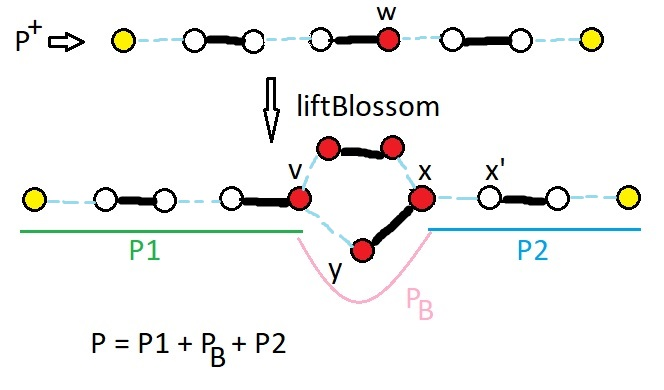
\includegraphics[scale=0.58]{lifting.jpg}
    \caption{Lifting a Blossom}
\end{figure}


\section{Proof of Correctness}
\subsection{Lemmas}
\subsubsection{Augmenting Path Lemma}
Given a graph $G$, a matching $M$ is maximum if and only if there is no augmenting path in $G$.

This lemma has been proved in lecture so we use it as it is.

\subsubsection{Identification Lemma}
Identification Lemma: This algorithm identifies Blossoms correctly.

The Blossom Recursion subroutine is executed only when the following conditions hold. This is because the conditions we impose before executing the said subroutine.
\begin{enumerate}
    \item Edge $(v, w)$ is unmarked.
    \item The parent of $v$ and $w$ is same i.e. $p_v = p_w$. Hence both are reachable from each other.
    \item Node $w$ is at an even distance from it's root $p_v$.
\end{enumerate}
Now there are 2 cases.
\begin{itemize}
    \item Case A: $v \in M$. 
        In this case $v$ must have been added to the list of terminal nodes by some other node and due to the structure of addToForest subroutine, we always add nodes which are at even distance from some original root of forest $F$. 
    \item Case B: $v \notin M$ or equivalently $v \in F$.
        In this case $v$ itself is a root and it's distance is 0, hence even.
\end{itemize}
Hence both $v$ and $w$ are at an even distance from $p_v$ and so the path that exists between them in $F$ is of even length. This path together with the edge $(v, w)$ forms a blossom.

\subsubsection{Base Lemma}
Since this blossom is formed of edges alternating in $M$ and length of the cycle is odd, there is exactly one node in blossom which is incident on 2 edges which are both absent in $M$ but present in the blossom. We call this vertex as the base of the blossom.

Stem Lemma: If the base is saturated by $M$, then the augmenting path $P^+$ which passes through the contracted blossom, passes through it such that it passes through the base.

The above lemma is true since, if it is not the case then it would imply that the vertex (which is not a base) is incident on 2 edges which are present in $M$ which contradicts the definition of $M$.

Note that in the figure above, node $v$ is the base of the blossom of size 5.

\subsection{Blossom Lemma}
Blossom Lemma: $G$ contains an augmenting path if and only if $G^+$ (the graph after contraction of blossom) contains an augmenting path.

Note that if the augmenting path in $G$ or $G^+$ doesn't pass through the blossom, then the proof is trivial since the path in both of them is exactly equal.

\subsubsection{Forward Proof}
There are 2 cases depending upon whether or not the blossom is internal to the augmenting path in $G^+$ or is an endpoint.
\begin{itemize}
    \item Case A: Blossom is internal to the augmenting path. 
        
        Observation $A_1$: Due to the base lemma proved above, there is one node which is the base (defined in lemma above) and hence the edge which enters into the blossom is in the matching.
        
        Observation $A_2$: Any other node is in the matching $M$ such that it's corresponding edge belongs to the matching and hence the edge which exits the blossom to the other end is not in the matching.
        
        From the above 2 observations, when the blossom is contracted into a single node, these 2 edges are alternating edges and hence the corresponding path in $G^+$ is augmenting.
    \item Case B: Blossom is an endpoint.
        
        Observation $A_2$ holds for this case also.
        
        Now since, the blossom is internal, the blossom becomes an unsaturated vertex since there is no edge incoming to this contracted blossom. 
        
        Hence we can say that the augmenting path in $G^+$ is aagain an augmenting path.
        
\end{itemize}


\subsubsection{Backward Proof}
Now since the blossom is of odd length, (WLOG) if we consider the base as the entry point and the other vertex as the exit point in the blossom, we can see that there are 2 paths (one travelling the upper path and the other travelling the lower path) between them. 

Independent of the position of the exit point wrt the entry point (base vertex), there is always a path of even length and a path of odd length. 

If we traverse from the base on the even length portion of the blossom, the first edge is not in the matching and the subsequent edges alternate. And since the path is of even length, the last edge is necessarily in matching.

Now again there are 2 cases.
\begin{itemize}
    \item Case A: Blossom is internal.
        
        According to the base lemma, the subpath outside the blossom attaching the unsaturated vertex to the base will end with an edge (incident on base) which is in the matching.
        
        For the edge connecting the exit point with the other unsaturated vertex, it is necessarily not in matching since the corresponding edge in matching $M$ belongs to the blossom.
        
        Hence in this case, the paths described above in union with the even length path forms an augmenting path in $G$.
    \item Case B: Blossom is and endpoint.
    
        For this case the first path in case A is an empty path and rest of the reasoning remains the same.
        
        Hence in this case also, the union of these paths forms an augmenting path in $G$.
\end{itemize}
Hence from the above Blossom Lemma in combination with the augmenting path lemma and the identification lemma, we can say that our algorithm is correct.

\section{Complexity Analysis}
\begin{itemize}
    \item The addToForest subroutine takes O(1) time since all 6 steps complete in constant time.
    \item The constructPath subroutine takes O($N$) time since the maximum length of a path can be $N$.
    \item The liftBlossom subroutine takes O($N$) time since the maximum length of the path can be $N$ and the decision to decide the subportion of the blossom to include in lifting the path is done in constant time.
    \item The findMaxMatching function is called recursively at max $\frac{N}{2}$ times since the size of the matching increases by 2 in every recursion call. Hence the time complexity is O$(N*$ cost of findAugmentingPath subroutine)
    \item Each call to the blossomRecursion subroutine will take at max O($N$) time since in each call the cost is equal to the size of the blossom found. The sum of size of all blossom cannot be more than $N$ since after each call the nodes are contracted and hence over counting cannot happen. Hence the top-level call will take O($N$) time.
    \item The number of iterations of loop over the edges in findAugmenting path is bound by $M$. See that addToForest subroutine takes O(1) time, constructPath subroutine takes O($N$) time and the blossomRecursion subroutine takes O$(N)$ time. Hence each iteration takes O$(1+N+N)$ = O($N$) time. Hence the time complexity is O$(M*N)$.
\end{itemize}

Finally plug the above result in time complexity of findMaxMatching function. Hence overall time complexity of the entire algorithm is O$(N * O(M*N)) = $ O($N^2M$).

\section{Parallel Blossom Algorithm}
Now in the core subroutine given below, the outer for loop which iterates over vertices $v$ can't be parallelised since after each iteration, the state of the tree changes and hence there is an inherent dependency. However the inner loop which iterates over the adjacent edges of some vertex $v$ can be done in parallel. However in the sequential version, after processing one edge, we may either find a path (without the need of a Blossom Recursion) or we find no augmenting path and there is some blossom or there is no augmenting path. So if we allow each iteration to modify the forest in parallel, the state of the forest becomes inconsistent if one iteration finds a path and other doesn't. Hence we have to delay the actual modification of the forest until all edges have been processed. Note that this implies that we can't use the AddToForest subroutine.

\begin{algorithm}[!h]
\caption{FindAugmentingPath}
\KwData{$G$, $M$}
\KwResult{$P$}

$F \leftarrow$ empty forest

rootOfNode $\leftarrow$ empty node-to-node mapping

terminals $\leftarrow$ unsaturated vertices of $G$

\For{each node $v$ in terminals}{
    rootOfNode($v$) $\leftarrow v$
    
    mark all edges of $M$ in $G$
    
    \textcolor{red}{temp $\leftarrow$ empty map}
    
    \For{each unmarked edge $(v, w)$ adjacent to $v$ \textcolor{red}{in PARALLEL}}{
        \uIf{$w \in M$}{
            \textcolor{red}{$x \leftarrow$ node adjacent to $w$ in $M$}
        
            \textcolor{red}{temp($w$) $\leftarrow x$}
        }\uElse{
            $p_w \leftarrow$ rootOfNode($w$)
            
            \If{$d(w, p_w)$ is even}{
                $p_v \leftarrow$ rootOfNode($v$)
                
                \uIf{$p_v$ == $p_w$}{
                    $P \leftarrow$ BlossomRecursion($G, M, F, v, w$)
                }\uElse{
                    $P \leftarrow$ ConstructPath($F, v, w$, rootOfNode)   
                }
                return $P$
            }
        }
        
        mark edge $(v, w)$    
    }
    
    \For{\textcolor{red}{each node $w$ in temp in PARALLEL}}{
        \uIf{\textcolor{red}{$w ==$ temp(temp($w$))}}{
            \textcolor{red}{$P \leftarrow$ BlossomRecursion($G, M, F, v, w$)}
            
            \textcolor{red}{return $P$}
        }\uElse{
            \textcolor{red}{add edges $(v, w)$ and $(w, \mathrm{temp}(w)=x)$ in $F$}
            
            \textcolor{red}{add node $x=\mathrm{temp}(w)$ to terminals}
        }
    }
}

return empty path
\end{algorithm}

The maximum matching wrapper depends on the previous matching and so can't be parallelised however augmenting a matching can be done in parallel.

\begin{algorithm}[H]
\SetAlgoLined
\caption{FindMaxMatching}

$P \leftarrow$ FindAugmentingPath($G$, $M$)

\If{$P$ is empty}{return $M$}

$M^+ \leftarrow$ increased matching of $M$ by adding alternating edges of $P$ \textcolor{red}{in PARALLEL}

return FindMaxMatching($G$, $M^+$)
\end{algorithm}

The construct path algorithm is sequential by nature and hence can't be parallelised. The best we can do is find $P_1 \& P_2$ in parallel. This doesn't scale as the number of processors increases.

\begin{algorithm}[!h]
\caption{ConstructPath}
\KwData{$F, v, w$, rootOfNode}
\KwResult{$P$}

$p_v \leftarrow$ rootOfNode($v$)

$p_w \leftarrow$ rootOfNode($w$)

$P_1 \leftarrow$ Path from $v$ to $p_v$ in forest $F$ \textcolor{red}{in PARALLEL with $P_2$}

$P_2 \leftarrow$ Path from $v$ to $p_w$ in forest $F$ \textcolor{red}{in PARALLEL with $P_1$}

return $P_1 + P_2$
\end{algorithm}

In the below algorithm, the once the blossom is found, the contraction of the blossom can be done in parallel since the presence of each edge in the blossom is independent from other edges. The lifting algorithm remains unchanged due to dependencies in the path finding process.

\begin{algorithm}[!h]
\caption{Blossom Recursion}
\KwData{$G, M, F, v, w$}
\KwResult{$P$}

$B \leftarrow$ nodes in path from $v \to w$ in $F$

$G^+ \leftarrow G$ with all nodes of $B$ contracted into $w$ \textcolor{red}{in PARALLEL}

$M^+ \leftarrow M$ with all nodes of $B$ contracted into $w$ \textcolor{red}{in PARALLEL}

$P^+ \leftarrow$ findAugmentingPath($G^+, M^+$)

\If{$w \in P^+$}{
    $P \leftarrow$ liftBlossom($B, P^+, M$)

    return $P$
}

return $P^+$
\end{algorithm}

\subsection{Proof of Correctness}
we will consider the parallelism seen in the augmenting path finding algorithm since we're deviating from the serial counterpart.

When extending the forest in parallel, we are only considering the effect of adding one unmarked edge at a time. Since when processed in isolation, if blossoms are formed due to addition of this single edge then our algorithm is no different from the serial counterpart in terms of behaviour. Hence, to prove the correctness our algorithm, we only need to consider the case when a blossom is formed due to addition of edges from the same node $v$.

Suppose two edges $(v, w_i)$ and $(v, w_j)$ are some two edges. Their corresponding marked edges are $(w_i, x_i)$ and $(w_j, x_j)$. Note that $x_i$ and $x_j$ are BOTH not present in the forest at this moment since if one of them were present then we would found a blossom while considering the other, before reaching at this situation. Both $(v, w_i)$ and $(v, w_j)$ are unmarked so $v$ is necessarily the base of the blossom. Now consider the following 2 cases:
\begin{itemize}
    \item Blossom is of size 5 or greater: If it is blossom of size 5 or more then the remaining part of the blossom should already be present in the forest since we have just added 3 edges and discovered a blossom. But this leads to a contradiction to our original assumption that $x_i$ and $x_j$ were both absent in the forest.
    \item Blossom is of size 3: From above, we can see that the blossom formed would always be a size 3 blossom. We are specifically checking for size 3 blossom in our algorithm after the edges are handled in parallel.
\end{itemize}

\subsection{Time Complexity}
\begin{itemize}
    \item There will be at max O($|V|$) iterations of the main algorithm since a matching of size at max $\frac{|V|}{2}$ is possible.
    \item We are now iterating over all the nodes hence there will be O($|V|$) iterations of the outer loop in the augmenting path finding algorithm. 
    \item Except the blossom recursion, the rest of task is done in constant time in each of the parallel iterations. For $p$ processors, it would take $\frac{|V|}{p}$ iterations. 
    \item In the blossom recursion, we are first constructing the blossom which is an O$(|V|)$ task when considering all the levels of the recursion. Once the blossom is constructed, the contraction can be done in parallel taking O($\frac{|E|}{p}$) time.
\end{itemize}
Hence the overall time complexity would be O($|V| \times |V| \times \frac{|V|}{p} \times (|V|+\frac{E}{p})$) = O$(|V|^3 + \frac{|V|^4}{p} + \frac{|V||E|}{|p|^2})$.

\section{References}
\begin{itemize}
    \item \href{https://stanford.edu/~rezab/classes/cme323/S16/projects_reports/shoemaker_vare.pdf}{\color{blue} Blossom Algorithm Analysis by Amy Shoemaker \& Sagar Vare (Clickable URL)}
    \item \href{https://en.wikipedia.org/wiki/Blossom_algorithm}{\color{blue} Wikipedia Blossom Algorithm (Clickable URL)}
\end{itemize}



\end{document}
